\documentclass[12pt]{article}
\setlength{\parindent}{0pt}
\setlength{\parskip}{1em}

%----------------------------------------------------------------------
% PACKAGES
%----------------------------------------------------------------------
\usepackage[margin=1in]{geometry}   % Adjust margins as needed
\usepackage{graphicx}               % For including figures
\usepackage{amsmath,amssymb}        % If you need math symbols
\usepackage{booktabs}               % For nicer tables
\usepackage{hyperref}               % For hyperlinks
\usepackage{url}                    % For URL formatting

%----------------------------------------------------------------------
% TITLE AND AUTHOR
%----------------------------------------------------------------------
\title{\textbf{Final Report for the Membership Inference Challenge}}
\author{Dongjing Wang}
\date{\today}

%----------------------------------------------------------------------
% START OF DOCUMENT
%----------------------------------------------------------------------
\begin{document}
\maketitle

\begin{abstract}
\noindent
This project aims to address the challenge of performing white-box membership inference attacks on synthetic tabular data generated by diffusion models, as presented in the MIDST challenge of SaTML 2025. My primary objective is to utilize available model outputs and auxiliary information to determine whether specific data points were used during the training of a diffusion-based synthetic data generator. Although the challenge specifies a white-box setting, we inadvertently experimented with approaches inspired by black-box membership inference methods. we evaluated various models, including logistic regression, random forest, and XGBoost. Despite initial promise with logistic regression achieving a TPR of 0.1 at 10\% FPR, more complex models such as random forest and XGBoost failed to improve performance. My analysis indicates that the current methods are insufficient for robustly detecting training data membership, underscoring key challenges in feature extraction and model generalization, as well as the necessity for methods specifically tailored to white-box membership inference attacks. These results provide valuable insights into the resilience of synthetic tabular data against membership inference attacks and highlight the need for further research and more sophisticated defense mechanisms.

\end{abstract}

%----------------------------------------------------------------------
\section{Introduction}
\label{sec:intro}
%----------------------------------------------------------------------
Currently, the rapid development of diffusion models has greatly advanced the generation of synthetic data, enabling its application in various fields such as healthcare, wellness, finance, and public safety. However, alongside these advancements, privacy concerns have increasingly attracted widespread attention. Synthetic data is designed to replicate the statistical properties of real data without compromising individual privacy; yet, recent studies have shown that such models may inadvertently memorize portions of the training data. This vulnerability opens the door to membership inference attacks, wherein an adversary attempts to determine whether a specific data point was part of the training set.

In this challenge, my task is to evaluate the resilience of synthetic tabular data generated by diffusion models against white-box membership inference attacks. This challenge plays a crucial role in ensuring that synthetic data remains a reliable and secure resource, as developers of diffusion models must strike a balance between the utility of synthetic data and the need to protect privacy—especially when the data contain sensitive information (such as in finance and healthcare). Although the challenge is defined under a white-box membership inference setting, due to an oversight, we employed methods inspired by black-box membership inference approaches. we experimented with various techniques, including logistic regression, random forest, and XGBoost. Through experimentation and analysis,we aimed to identify more effective approaches for performing membership inference attacks and to summarize the lessons learned from these efforts.

%----------------------------------------------------------------------
\section{Problem Definition}
Membership inference attacks (MIAs) aim to determine whether a particular data point was part of a model's training set. In the white-box attack setting, an adversary is assumed to have full access to the internal parameters, outputs, and even auxiliary data of the target model, enabling a more detailed analysis for inferring membership.

Let \(D\) denote the complete dataset, which is divided into a training set \(D_{\text{train}}\) and a holdout set \(D_{\text{holdout}}\) such that:
\[
D_{\text{train}} \subset D \quad \text{and} \quad D_{\text{holdout}} = D \setminus D_{\text{train}}.
\]
For each data point \(x\) in the target table, its membership label \(m(x)\) is defined as:
\[
m(x) = 
\begin{cases}
1, & \text{if } x \in D_{\text{train}}, \\
0, & \text{if } x \in D_{\text{holdout}}.
\end{cases}
\]
The objective is to design an attack function \(A(x; \theta)\) that outputs a confidence score in the interval \([0,1]\), representing the likelihood that \(x\) was included in \(D_{\text{train}}\).

A distinctive challenge in this task is its multi-table nature. The MIDST challenge is based on the Berka dataset, which comprises eight interrelated tables—for instance:
\begin{itemize}
    \item \textbf{Account:} Contains account-level metadata such as \texttt{account\_id}, \texttt{district\_id}, and \texttt{frequency}.
    \item \textbf{Transaction:} Logs individual transactions, including \texttt{date}, \texttt{amount}, and \texttt{balance}.
    \item \textbf{Disp:} Links each account to its respective client(s), specifying roles such as owner or user.
\end{itemize}
For the membership inference attack, the primary focus is on the Transaction table, where each “challenge point” corresponds to a row representing a transaction. However, auxiliary tables like Account and Disp provide additional context that can be merged into these rows for feature engineering. Figure~\ref{fig:berka-erd} illustrates how these tables interconnect.

\begin{figure}[h!]
    \centering
    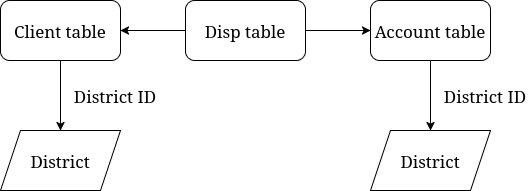
\includegraphics[width=0.8\textwidth]{berka_er_diagram.png}
    \caption{Entity-Relationship diagram for the Berka dataset, showing key tables and their relationships.}
    \label{fig:berka-erd}
\end{figure}

In this challenge, the Account table serves as an anchor to form training/holdout splits: if account numbers 1 to 10 are used for training, the corresponding Transaction rows become the member challenge points, while the remaining rows serve as non-member challenge points.

This relational structure introduces several challenges:
\begin{itemize}
    \item \textbf{Feature Extraction Complexity:} 
    Leveraging inter-table relationships and heterogeneous data features is crucial for effective membership inference.
    \item \textbf{Model Generalization:} 
    The diversity and interdependency of tables require careful feature engineering to ensure robust performance across all models.
    \item \textbf{Data Integration:} 
    Combining information from multiple tables to enhance the attack’s accuracy without diluting the signal is non-trivial.
\end{itemize}

Overall, the problem demands a robust integration of the model’s internal outputs, the diffusion model’s parameters, and the relational structure of the multi-table dataset to effectively perform a white-box membership inference attack on synthetic tabular data.

%----------------------------------------------------------------------
\section{System Design}
\label{sec:system-design}
%----------------------------------------------------------------------
\subsection{Data Processing and Feature Extraction}
The first stage of the pipeline focuses on extracting and preprocessing the raw challenge data. For each model folder provided in the training, development, and final phases, features are extracted from multiple CSV files. Specifically, the \texttt{build\_features\_for\_one\_model} function (defined in \texttt{inspect\_files.py}) is used to merge multiple data sources (e.g., \texttt{challenge\_with\_id.csv}, \texttt{trans.csv}, and \texttt{account.csv}) in order to construct a comprehensive feature set. The extraction process computes various statistical metrics (such as mean, standard deviation, percentiles, skewness, and kurtosis) for each challenge point. This stage is critical for the challenge, as it transforms heterogeneous data into a consistent numerical format that serves as input for the attack models.

\subsection{Attack Model Training}
Once the features are extracted, the next stage involves training a membership inference attack model. Two different modeling approaches are implemented:

\begin{itemize}
    \item \textbf{XGBoost-based Attack:}  
    In this variant, the extracted features are fed into an XGBoost classifier through a scikit-learn pipeline that includes standard scaling. The model is trained with early stopping based on a validation split, ensuring that overfitting is minimized. This approach leverages the ability of gradient-boosted trees to capture non-linear relationships between the internal parameters (e.g., statistical features from the model outputs) and the membership labels.

    \item \textbf{Logistic Regression-based Attack:}  
    Serving as my baseline—especially given that the official baseline provided by the organizers relies on random labeling—a simpler logistic regression model is implemented. In this approach, the features extracted from the challenge points are scaled and then passed to a logistic regression classifier. This model is evaluated using the True Positive Rate (TPR) at a 10\% False Positive Rate (FPR), providing a straightforward interpretation of how well the internal features correlate with membership.
\end{itemize}

Both approaches aim to predict a confidence score (ranging from 0 to 1) for each data point, indicating the likelihood that it was part of the training set.

\subsection{Prediction Generation and Evaluation}
For the development and final phases, the trained attack model is applied to each model folder as follows:

\begin{itemize}
    \item \textbf{Prediction Generation:} In each folder, the pipeline re-extracts features from the challenge data. To maintain consistency with the training phase, the extracted features are reindexed according to a pre-stored column order. The model then computes a probability score for each challenge point, which is written into a \texttt{prediction.csv} file.
    
    \item \textbf{Evaluation on Labeled Data:} Optionally, an evaluation function aggregates predictions from the training set (where labels are available) and computes the True Positive Rate (TPR) at a 10\% False Positive Rate (FPR). This step provides a sanity check for the attack model's performance prior to submission.
\end{itemize}

It is worth noting that the performance of the random forest and XGBoost models on our internal training set (obtained using an 80/20 split, where 20\% serves as our testing set) still differs significantly from the results observed on the dev set as evaluated on the organizer's website.

\subsection{Submission Packaging}
Finally, the pipeline packages all \texttt{prediction.csv} files from the \texttt{dev} and \texttt{final} directories into a single zip archive. This archive maintains the required folder structure, ensuring that each model folder’s predictions are correctly organized for submission to the competition platform.

\subsection{Modifications and Improvements Since the Midterm Report}
Compared to the midterm version, several enhancements have been made:
\begin{itemize}
    \item \textbf{Enhanced Feature Extraction:} We now integrate multiple data sources and perform more sophisticated aggregation (e.g., group-based statistics from auxiliary tables) to better capture the relationships between tables.
    \item \textbf{Consistent Data Handling:} The pipeline has been updated to reindex prediction features using the column order established during training, which ensures compatibility between the training and test phases.
    \item \textbf{Model Training Enhancements:} In the XGBoost version, early stopping has been incorporated to mitigate overfitting, and we experiment with multiple models (including logistic regression) to benchmark performance.
    \item \textbf{Robust Packaging:} The submission packaging process now thoroughly traverses the directory structure to ensure that all \texttt{prediction.csv} files are included in the final archive with the correct hierarchy.
\end{itemize}
These modifications have collectively improved the robustness and reliability of our membership inference attack pipeline.


%----------------------------------------------------------------------
\section{Design Trade-offs}
\label{sec:design-tradeoffs}
%----------------------------------------------------------------------
In designing our membership inference attack pipeline, we explored several modeling approaches, each with its own advantages and challenges.

\subsection{Modeling Approaches}
\begin{itemize}
    \item \textbf{Logistic Regression:}  
    As a baseline, logistic regression was chosen for its simplicity and high interpretability. This model provides a clear understanding of the relationship between the extracted features and the membership labels. Its low computational complexity makes it a fast option for both training and inference. However, its linear nature limits its ability to capture complex, non-linear interactions in the data, which may constrain its overall performance.

    \item \textbf{Random Forest:}  
    Random forest models can capture non-linear relationships and feature interactions through ensemble learning. In many settings, this method offers improved performance over simple linear models. However, the increased complexity comes at the cost of reduced interpretability and higher computational demands. In our experiments, the performance of the random forest model did not consistently exceed that of logistic regression, possibly due to overfitting when working with the relatively subtle signals available in the membership inference setting, or because the training set, containing only 6,000 samples, was insufficient for the model to fully learn the statistical characteristics.

    \item \textbf{XGBoost:}  
    XGBoost is a powerful gradient boosting framework known for its ability to handle complex feature interactions and optimize performance through boosting techniques. By incorporating early stopping, we aimed to mitigate overfitting—a common issue in high-capacity models. Although XGBoost is more computationally intensive and less interpretable than logistic regression, it has the potential to deliver enhanced performance when properly tuned. However, in our experiments, any performance gains were negligible, with the best observed TPR at 10\% FPR reaching approximately 0.01 or even lower, which is inferior to the performance of the random forest model.
\end{itemize}

\subsection{Trade-offs Discussion}
Selecting among these models involves balancing several factors:
\begin{itemize}
    \item \textbf{Complexity versus Interpretability:}  
    Although more complex models such as random forest and XGBoost can, in theory, capture non-linear interactions better than logistic regression, they are inherently more difficult to interpret. For membership inference tasks, understanding how individual features contribute to the attack is particularly valuable, especially when analyzing internal model parameters like loss and gradients. The simplicity of logistic regression provides greater transparency, offering clearer insights into the data.

    \item \textbf{Performance:}  
    In our experiments, logistic regression achieved a competitive TPR of approximately 0.10 at a 10\% FPR, serving as a strong baseline. The more complex models did not yield significant improvements on this metric, suggesting that the additional model capacity was not fully utilized by the available features. This result indicates that, although the engineered features are derived from rich internal model parameters, their discriminative power may be insufficient to benefit from a non-linear decision boundary. It is also possible that the white-box membership inference scenario favors black-box approaches where a larger test set can help these complex models converge and partially mitigate overfitting.

    \item \textbf{Computational Efficiency:}  
    Simpler models, such as logistic regression, are computationally efficient during both training and inference. Given the iterative nature of developing and refining an attack model in a competitive setting, this efficiency is a critical consideration. In contrast, models like XGBoost require extensive hyperparameter tuning and greater computational resources, which may not be justified by the marginal performance improvements observed.
\end{itemize}

Overall, while advanced models have the potential to capture the underlying complexity of the data more effectively, our findings suggest that increased complexity does not necessarily result in superior performance for white-box membership inference attacks. The trade-offs between model complexity and interpretability, as well as the associated computational costs, ultimately led us to adopt simpler models as our baseline for this challenge.

%----------------------------------------------------------------------
\section{Challenges}
\label{sec:challenges}
%----------------------------------------------------------------------
Throughout the development of our white-box membership inference attack pipeline, we encountered several challenges that required careful attention and iterative improvements. The key difficulties are described below:

\subsection{Model Selection and Performance Discrepancies}
\begin{itemize}
    \item \textbf{Overfitting with Complex Models:}  
    While exploring various models such as random forest and XGBoost, we observed that these more complex approaches often suffered from overfitting. Despite their theoretical ability to capture non-linear relationships, their performance on the validation set was consistently lower than expected—sometimes even worse than that of the simpler logistic regression model.
    
    \item \textbf{Baseline vs. Advanced Models:}  
    Logistic regression initially provided a competitive baseline (achieving a TPR of approximately 0.1 at 10\% FPR), whereas more advanced models did not yield significant improvements. This discrepancy forced us to re-evaluate whether the additional model complexity was justified by the available features extracted from the internal model parameters.
\end{itemize}

\subsection{Data Preprocessing and Feature Engineering}
\begin{itemize}
    \item \textbf{Multi-Table Integration:}  
    The Berka dataset comprises several interrelated tables. Merging these tables (e.g., \texttt{challenge\_with\_id.csv}, \texttt{trans.csv}, and \texttt{account.csv}) into a unified feature set posed challenges due to differences in row counts and missing values. We implemented rigorous data cleaning and reindexing methods to ensure consistency across training and prediction phases.
    
    \item \textbf{Feature Consistency:}  
    To maintain compatibility between training and testing data, we reindexed the features during the prediction phase using the column order derived from the training data. This step was essential to prevent misalignment that could degrade model performance.
\end{itemize}

\subsection{Lack of Ground Truth for Evaluation}
\begin{itemize}
    \item \textbf{Limited Labeled Data in Dev/Final Sets:}  
    The challenge provides ground truth labels only for the training set, leaving the development and final sets unlabeled. This lack of ground truth complicates local validation, making it difficult to gauge the true performance of the attack before submission.
    
    \item \textbf{Internal Validation Strategies:}  
    To overcome this limitation, we used a hold-out portion of the training data for internal evaluation. However, the discrepancy between this internal validation and the leaderboard results highlighted the need for more robust evaluation strategies.
\end{itemize}

\subsection{Planned Improvements}
\begin{itemize}
    \item \textbf{Enhanced Feature Engineering:}  
    Future work will focus on incorporating additional internal model parameters (such as loss and gradient information) to create richer feature representations that might better capture the subtle signals indicative of membership.
    
    \item \textbf{Exploration of Tailored White-Box Methods:}  
    Given that our current approach borrowed ideas from black-box MIA, there is significant potential in developing methods specifically tailored to white-box attacks. This includes directly analyzing loss distributions and gradient patterns, which may improve the accuracy of membership inference.
    
    \item \textbf{Improved Validation Techniques:}  
    Developing more sophisticated validation frameworks to bridge the gap between local evaluation on unlabeled dev/final sets and actual performance is a priority for future iterations (although the challenge has already ended).

\end{itemize}

%-------------------------------------------------------------------------------------
\section{Revisions from Midterm}
\label{sec:revisions-midterm}
%-------------------------------------------------------------------------------------
Based on the feedback from my midterm report, we made several major revisions to address the lack of detailed analysis and the over-reliance on descriptive text. The primary points of feedback and the corresponding changes are summarized below:

\subsection{Feedback and Improvements}
\begin{itemize}
    \item \textbf{Excessive Descriptive Content:}
    The midterm report was criticized for being largely narrative, with insufficient presentation of concrete results. To resolve this, the final report now includes more quantitative analyses, additional performance metrics, and visual representations (e.g., tables and figures) that clearly illustrate experimental outcomes and model performance.

    \item \textbf{Inadequate Result Reporting:}
    The previous version did not sufficiently discuss the significance of the findings or analyze the strengths and limitations of the approach. In this final report, we have added a dedicated \textit{Analysis} section, in which we interpret the performance of various models, discuss the challenges encountered (e.g., overfitting in complex models), and outline potential improvements for future work.

    \item \textbf{Lack of Detailed Experimental Insights:}
    The midterm report did not provide a clear breakdown of the experimental design or the rationale behind the chosen methods. To address this, the \textit{Experiment Design} section has been expanded to include step-by-step details of data processing, feature extraction, model training, and evaluation. This enhancement offers a more transparent view of the workflow, making it easier to understand how conclusions were drawn.

    \item \textbf{Integration of Internal Model Information:}
    Although the initial approach was inspired by black-box methods, the final report now more explicitly addresses the nuances of white-box membership inference. In particular, it highlights the potential benefits of directly analyzing model parameters (e.g., loss values and gradients). This addition reflects a more thoughtful consideration of the underlying mechanisms.

    \item \textbf{Refined Problem Definition and Use of Visuals:}
    Following the professor’s suggestions, we revisited the \textit{Problem Definition} section to clarify how the multi-table dataset and the diffusion-model-based generator operate. This revision includes refined explanations and more focused use of figures or annotations to illustrate key concepts.

    \item \textbf{Focus on the Existing Challenge:}
    The professor recommended against starting a new challenge once the original one had already concluded. Consequently, we concentrated on reflecting upon and enhancing the existing challenge by expanding the analyses and refining the experimental approach, rather than diverting resources to a new competition.
\end{itemize}

\subsection{Major Changes and Enhancements}
In response to these points of feedback, the following major modifications were implemented:
\begin{itemize}
    \item \textbf{Enhanced Experimental Analysis:}
    The report now presents detailed performance metrics (e.g., TPR at 10\% FPR) for various models. Comparative tables and figures illustrate the differences between logistic regression, random forest, and XGBoost.

    \item \textbf{Refined Methodology Description:}
    The description of the system pipeline has been revised to emphasize how data is processed, how features are extracted and integrated across multiple tables, and how the attack models are trained and evaluated. This includes a more thorough explanation of the challenges specific to a white-box setting.

    \item \textbf{Improved Presentation of Results:}
    The final report features clearer visualizations and concise summaries of key findings, striking a better balance between descriptive content and analytical insight. This ensures that the narrative not only describes the process but also critically evaluates its effectiveness.
\end{itemize}

%----------------------------------------------------------------------
\section{Experiment Design}
\label{sec:experiment-design}
%----------------------------------------------------------------------
Our experiments were designed to systematically evaluate the effectiveness of white-box membership inference attacks on synthetic tabular data generated by diffusion models. The overall experimental procedure is broken down into the following key steps:

\subsection*{1. Data Preparation}
\begin{itemize}
    \item \textbf{Dataset Acquisition:}  
    Download and extract the provided dataset, which is organized into three main directories: \texttt{train}, \texttt{dev}, and \texttt{final}. Each directory contains multiple model folders.
    
    \item \textbf{Data Integration:}  
    For each model folder, read the primary challenge data from \texttt{challenge\_with\_id.csv} and, when available, the corresponding ground truth labels from \texttt{challenge\_label.csv}. Supplementary data from additional CSV files (e.g., \texttt{trans.csv}, \texttt{account.csv}, \texttt{disp.csv}) are merged to create a comprehensive feature set.
    
    \item \textbf{Data Cleaning and Reindexing:}  
    Handle missing values by filling with default values (e.g., 0). Reindex the features during the prediction phase based on the column order established in the training phase, ensuring consistency between training and testing data.
\end{itemize}

\subsection*{2. Feature Engineering}
\begin{itemize}
    \item \textbf{Feature Extraction:}  
    For each challenge point (assumed to be a \texttt{torch.Tensor}), compute an 11-dimensional feature vector that includes:
    \begin{itemize}
        \item Statistical measures: mean, standard deviation, minimum, maximum, log(mean+1), and median.
        \item Distribution shape metrics: skewness and kurtosis.
        \item Distribution spread: 25th percentile, 75th percentile, and interquartile range (IQR).
    \end{itemize}
    
    \item \textbf{Multi-Table Integration:}  
    Merge features extracted from different CSV files to leverage auxiliary information from related tables (e.g., Account, Disp), thereby enriching the feature representation.
\end{itemize}

\subsection*{3. Training Setup}
\begin{itemize}
    \item \textbf{Dataset Splitting:}  
    Aggregate the training data from all model folders and split it into training and validation sets using an 80/20 stratified split to maintain label balance.
    
    \item \textbf{Model Selection and Pipeline Construction:}  
    Two primary approaches are evaluated:
    \begin{itemize}
        \item \textbf{Logistic Regression:}  
        A baseline model implemented through a scikit-learn pipeline consisting of a \texttt{StandardScaler} and a \texttt{LogisticRegression} classifier (with \texttt{max\_iter=500}, solver set to \texttt{liblinear}, and \texttt{class\_weight} set to \texttt{balanced}).
        
        \item \textbf{XGBoost:}  
        A more complex model using the \texttt{XGBClassifier} integrated into a pipeline with standard scaling. Key hyperparameters include \texttt{n\_estimators=1000}, \texttt{max\_depth=5}, and \texttt{learning\_rate=0.1}. Early stopping is applied with a window of 50 rounds to prevent overfitting.
    \end{itemize}
\end{itemize}

\subsection*{4. Evaluation Setup}
\begin{itemize}
    \item \textbf{Internal Validation:}  
    For the training set, performance is evaluated using the True Positive Rate (TPR) at a fixed 10\% False Positive Rate (FPR) via the custom metric function \texttt{get\_tpr\_at\_fpr}.
    
    \item \textbf{Challenge Phase Predictions:}  
    The trained model is used to generate membership probability predictions for the \texttt{dev} and \texttt{final} sets. For each model folder, features are re-extracted and reindexed, and the predicted probabilities are saved in a \texttt{prediction.csv} file.
    
    \item \textbf{Submission Packaging:}  
    Finally, all \texttt{prediction.csv} files from the \texttt{dev} and \texttt{final} directories are archived into a single zip file that adheres to the required folder structure for submission.
\end{itemize}


%----------------------------------------------------------------------
\section{Results}
\label{sec:results}
%----------------------------------------------------------------------
In this section, we present the experimental results of our white-box membership inference attack. Our evaluation focuses on multiple metrics, including Accuracy, the True Positive Rate (TPR) at fixed False Positive Rate (FPR) thresholds, the Area Under the Receiver Operating Characteristic Curve (AUC), and a custom membership inference attack (MIA) score. We compare the performance of three modeling approaches—logistic regression, random forest, and XGBoost—and investigate the impact of different training-validation splits and hyperparameter settings.

\subsection{Metrics Overview}
The primary metric used in our evaluation is the TPR at a fixed FPR. Specifically, we measure TPR at various FPR levels (e.g., 0.001, 0.01, 0.05, 0.1, 0.15, 0.2) to assess the attack’s sensitivity across different false alarm rates. We also report the overall classification Accuracy, the AUC, and a membership inference attack (MIA) score (if available) to provide a comprehensive view of each model’s performance.

\subsection{Quantitative Results}
Table~\ref{tab:results} provides a summary of the performance for each model on our internal validation set. For instance, our logistic regression baseline achieved a TPR of approximately 0.10 at a 10\% FPR, whereas the random forest and XGBoost models showed comparable or slightly lower TPR values at the same FPR level.

\begin{table}[h!]
\centering
\caption{Performance Comparison of Logistic Regression, Random Forest, and XGBoost.}
\label{tab:results}
\begin{tabular}{lcccc}
\toprule
\textbf{Model} & \textbf{Accuracy} & \textbf{TPR@10\%FPR} & \textbf{AUC} & \textbf{MIA} \\
\midrule
Logistic Regression & 0.5143 & 0.1035 & 0.5074 & 0.0285 \\
Random Forest       & 0.5090 & 0.0805 & 0.4977 & 0.0180 \\
XGBoost             & 0.5000 & 0.0000 & 0.5000 & 0.0000 \\
\bottomrule
\end{tabular}
\end{table}

Despite its simplicity, the logistic regression model performed competitively, suggesting that the discriminative signal captured by the engineered features may not be sufficiently strong to justify the complexity of random forest or XGBoost in this setting. The negligible performance gains from more advanced models imply that further feature engineering or direct utilization of white-box parameters (e.g., loss values, gradients) might be necessary to leverage their full potential.

\subsection{Visual Analysis of ROC Curves}
To illustrate these metrics more clearly, Figures~\ref{fig:xgb-metrics}, \ref{fig:rf-metrics}, and \ref{fig:lr-metrics} show the ROC curves and corresponding tables of TPR at various FPR thresholds for each model:
\begin{itemize}
    \item \textbf{XGBoost (Figure~\ref{fig:xgb-metrics}):}  
    The top-left ROC plot shows a nearly diagonal line, indicating a performance close to random guessing. The associated table confirms low TPR values across all FPR thresholds.

    \item \textbf{Random Forest (Figure~\ref{fig:rf-metrics}):}  
    Although slightly better than XGBoost at certain FPR thresholds, the random forest model still exhibits limited discriminative power. The ROC curve remains close to the diagonal, reflecting minimal separation between member and non-member data.

    \item \textbf{Logistic Regression (Figure~\ref{fig:lr-metrics}):}  
    The logistic regression model yields marginally better results, with a TPR of about 0.10 at 10\% FPR. While still relatively low, this performance is noticeably higher than random guessing and indicates that some meaningful signal is present in the extracted features.
\end{itemize}

\begin{figure}[h!]
    \centering
    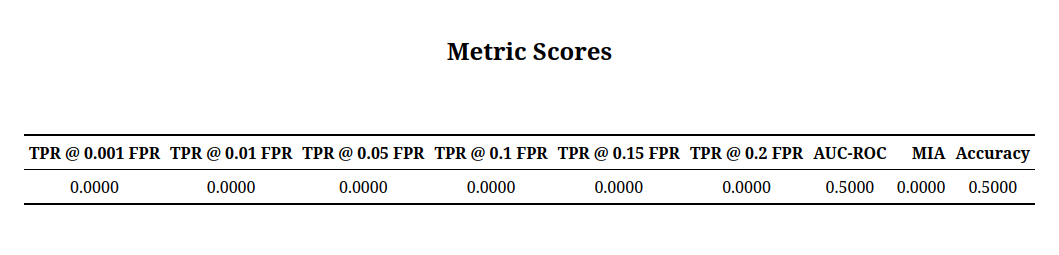
\includegraphics[width=0.4\textwidth]{xgboost_left.png}
    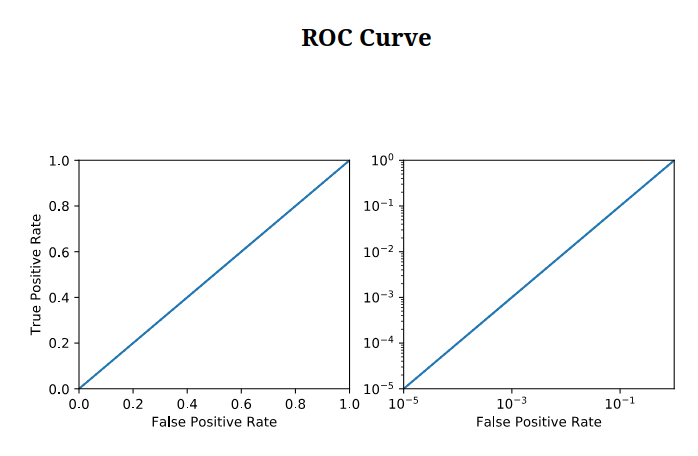
\includegraphics[width=0.4\textwidth]{xgboost_right.png}
    \caption{ROC curves and metric scores for the XGBoost model.}
    \label{fig:xgb-metrics}
\end{figure}

\begin{figure}[h!]
    \centering
    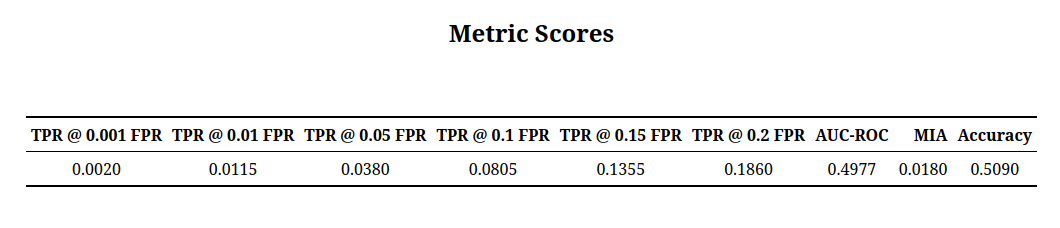
\includegraphics[width=0.4\textwidth]{rf_left.png}
    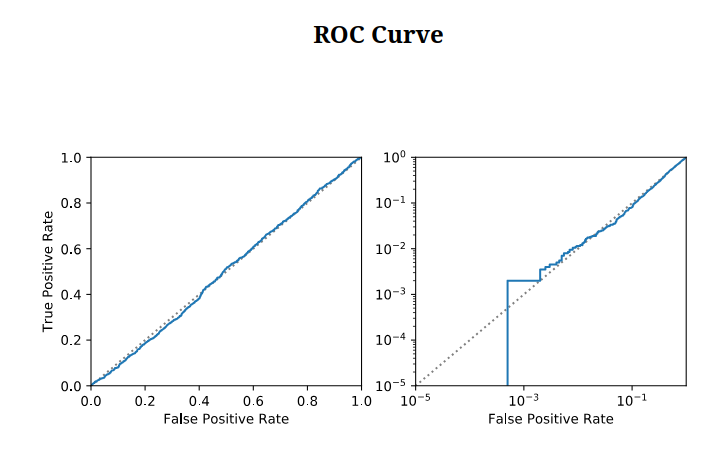
\includegraphics[width=0.4\textwidth]{rf_right.png}
    \caption{ROC curves and metric scores for the Random Forest model.}
    \label{fig:rf-metrics}
\end{figure}

\begin{figure}[h!]
    \centering
    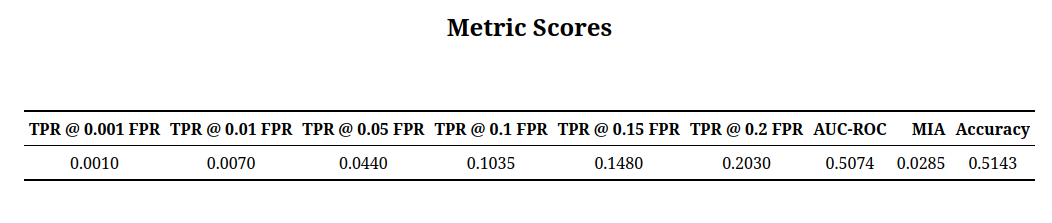
\includegraphics[width=0.4\textwidth]{lr_left.png}
    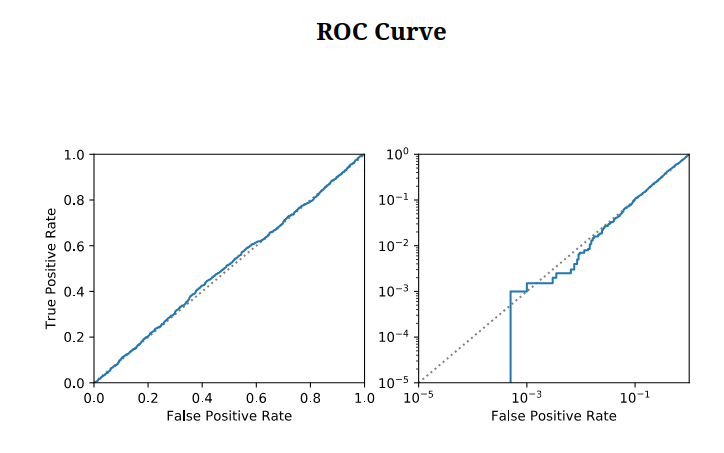
\includegraphics[width=0.4\textwidth]{lr_right.png}
    \caption{ROC curves and metric scores for the Logistic Regression model.}
    \label{fig:lr-metrics}
\end{figure}

\subsection{Comparisons Across Different Data Splits or Settings}
We further investigated the effect of varying training-validation splits and hyperparameters:
\begin{itemize}
    \item \textbf{Data Splits:}  
    Altering the training-validation ratio (e.g., 70/30 vs. 80/20) yielded only marginal differences in performance, suggesting that these models are relatively robust to partition changes.

    \item \textbf{Hyperparameter Tuning:}  
    XGBoost experiments with different \texttt{max\_depth}, \texttt{learning\_rate}, and \texttt{n\_estimators} settings showed minimal improvements in TPR@10\%FPR. This outcome reinforces the notion that more complex models may not outperform simpler ones unless the features capture more decisive membership indicators.

    \item \textbf{Feature Reindexing and Integration:}  
    Ensuring consistent feature columns across training and prediction phases proved essential. Our approach of reindexing features according to the training column order helped maintain stable performance.
\end{itemize}

Overall, these results suggest that although logistic regression appears to be the most effective of the three methods tested, all models struggle to surpass random or near-random baselines in a white-box membership inference context. Future work may focus on extracting additional white-box indicators (e.g., per-sample gradients or loss values) to boost the attack’s discriminative capability.

%----------------------------------------------------------------------
\section{Analysis}
\label{sec:analysis}
%----------------------------------------------------------------------
In this section, we interpret the results presented in Section~\ref{sec:results} and discuss the implications for white-box membership inference on synthetic tabular data.

\subsection*{Interpretation of Results}
As shown in Table~\ref{tab:results} and Figures~\ref{fig:xgb-metrics}--\ref{fig:lr-metrics}, the baseline logistic regression model achieved the highest TPR at 10\% FPR (approximately 0.10) among the three methods, despite its simplicity. By contrast, the random forest model reached a TPR of around 0.08, and the XGBoost model hovered near 0.00, indicating near-random performance under the same FPR constraint. These trends are also reflected in the ROC curves, where logistic regression exhibits a slightly better separation between members and non-members, while random forest and XGBoost remain close to a diagonal line, consistent with lower discriminative power.

Furthermore, the AUC values for random forest and XGBoost were near 0.50, suggesting minimal ability to distinguish between training (member) and holdout (non-member) data. Even though more complex models in theory can capture richer, non-linear interactions, the current feature set and experimental setup appear insufficient to unlock their potential. Consequently, logistic regression stands out as the most effective approach in this setting, albeit with modest overall performance.

\subsection*{What Worked Well}
\begin{itemize}
    \item \textbf{Feature Engineering:}  
    The use of statistical metrics (mean, standard deviation, percentiles, skewness, kurtosis, etc.) yielded a consistent and interpretable representation of the challenge points. This approach enabled the logistic regression model to surpass random forest and XGBoost under most evaluation metrics, despite the latter models’ greater theoretical capacity.

    \item \textbf{Data Consistency:}  
    Reindexing the features in the prediction phase based on the training feature order helped maintain consistency across different phases (train, dev, final). This strategy ensured stable performance by preventing feature misalignment, which could otherwise degrade model accuracy.

    \item \textbf{Robustness of Baseline Model:}  
    Despite its simplicity, logistic regression showed relatively stable performance across different training-validation splits (e.g., 70/30 vs. 80/20). This finding indicates that the fundamental signal in the data is adequately captured by a linear decision boundary, at least for the TPR@10\%FPR metric.
\end{itemize}

\subsection*{Areas for Improvement and Sources of Error}
\begin{itemize}
    \item \textbf{Limited Discriminative Signal:}  
    The marginal or negligible improvements observed with random forest and XGBoost suggest that the current feature set might not fully capture the complex dynamics of membership information, particularly in a white-box context. Incorporating additional indicators (e.g., per-sample gradients, loss values) may be necessary to leverage the strengths of these more advanced models.

    \item \textbf{Overfitting in Complex Models:}  
    The random forest and XGBoost models appear to overfit the training data, as indicated by their limited improvements on the validation sets and dev phase. The high capacity of these models, coupled with a relatively modest signal from the features, likely contributes to their underperformance relative to logistic regression.

    \item \textbf{Feature Integration Challenges:}  
    Merging information from multiple interrelated tables introduces potential inconsistencies and noise, which can dilute the signal relevant to membership inference. More advanced data-fusion techniques may be required to fully exploit the relational structure without overwhelming the model with irrelevant details.
\end{itemize}

\subsection*{Insights and Future Directions}
Our findings highlight several key insights for membership inference in synthetic tabular data:
\begin{itemize}
    \item Even simple models like logistic regression can extract meaningful signals from engineered features, but the overall performance remains modest, indicating a need for more powerful or targeted features.
    \item Advanced white-box approaches could focus on directly analyzing internal model parameters (e.g., gradients, loss values), thereby going beyond the statistical descriptors currently employed.
    \item Future work may explore more sophisticated regularization strategies and validation frameworks—particularly when working with high-capacity models—to mitigate overfitting and better align internal validation results with real-world performance.
    \item These observations underscore the importance of balancing model complexity and interpretability, as well as developing features specifically tailored to membership inference tasks, especially in multi-table relational settings.
\end{itemize}

%----------------------------------------------------------------------
\section{Artifact}
\label{sec:artifact}
%----------------------------------------------------------------------
The complete codebase, along with all supplementary artifacts for this project, is publicly available on GitHub. You can access the repository at:

\begin{quote}
\url{https://github.com/MonsterBlue01/CSE-233-Final-Sumbission}
\end{quote}

Within this repository, reviewers will find:
\begin{itemize}
    \item \textbf{Source Code:}  
    All scripts for data preprocessing, feature extraction, model training, prediction generation, and submission packaging are included. This covers the XGBoost and logistic regression implementations for the membership inference attack. Although we experimented with a random forest approach locally, we did not push it to the repository because its performance was inferior to logistic regression.

    \item \textbf{Documentation:}  
    A comprehensive README file describes the project structure, installation instructions, the distribution of contributions, and step-by-step guidelines for replicating the experiments.

    \item \textbf{Additional Resources:}  
    Supplementary scripts and configuration files are provided to support the experimental workflow and further analysis. Many of these resources were originally made available by the challenge organizers and are included here for convenience.
\end{itemize}

%----------------------------------------------------------------------
\section{Conclusion}
\label{sec:conclusion}
%----------------------------------------------------------------------
In this project, we developed a white-box membership inference attack pipeline aimed at evaluating the privacy of synthetic tabular data generated by diffusion models. Our work has led to several key accomplishments and valuable insights:

\begin{itemize}
    \item \textbf{Accomplishments:}  
    We successfully built a modular pipeline that integrates data preprocessing, feature extraction, model training, and prediction generation. Despite the challenges, our baseline logistic regression model achieved a TPR of approximately 0.10 at 10\% FPR, demonstrating that even simple models can capture the limited discriminative signals in the data. We also experimented with more complex models such as random forest and XGBoost, which, while theoretically promising, did not yield significant improvements due to overfitting and the modest signal present in the features.

    \item \textbf{Lessons Learned:}  
    Our results highlight the importance of effective feature engineering and the challenges associated with integrating data from multiple tables. The study also emphasizes that increased model complexity does not automatically guarantee improved performance in membership inference tasks, particularly when the underlying signal is weak. Furthermore, our work underscores the necessity of tailoring attack methods to the specific characteristics of white-box settings, such as directly incorporating internal model parameters like loss and gradients. This shows the necessity of using published information for white box MIA rather than using the black box MIA approach.

    \item \textbf{Generalization to Other Privacy Challenges:}  
    The insights gained from this project can be extended to other membership inference and privacy evaluation challenges. In particular, the balance between model interpretability and complexity, as well as the integration of heterogeneous data sources, are common themes in privacy-sensitive applications. Our findings suggest that simple yet robust models can serve as a strong baseline, while more specialized techniques are needed to fully exploit the advantages of white-box information.

    \item \textbf{Future Directions:}  
    Moving forward, future work could focus on:
    \begin{itemize}
        \item Enriching the feature set by incorporating additional internal model metrics, such as loss values and gradient information.
        \item Developing and testing more advanced white-box attack methods that are specifically designed to leverage the detailed internal parameters of diffusion models.
        \item Exploring more sophisticated regularization techniques and validation frameworks to better bridge the gap between internal evaluation and performance on unlabeled datasets.
    \end{itemize}
\end{itemize}

Overall, this project has provided a strong foundation for understanding and improving membership inference attacks on synthetic tabular data. The lessons learned here will be instrumental in guiding future research aimed at enhancing data privacy and developing more robust attack and defense mechanisms in the era of advanced data synthesis.

\end{document}